\documentclass[11pt]{article}

\usepackage[margin=1in]{geometry}
\usepackage[T1]{fontenc}
\usepackage[utf8]{inputenc}
\usepackage{lmodern}
\usepackage{microtype}
\usepackage{booktabs}
\usepackage{array}
\usepackage{longtable}
\usepackage{tabularx}
\usepackage{graphicx}
\usepackage{xcolor}
\usepackage{hyperref}
\usepackage{enumitem}
\usepackage{listings}
\usepackage{pgfplots}
\usepackage{float}
\usepackage{titlesec}

\pgfplotsset{compat=1.18}
\hypersetup{colorlinks=true,linkcolor=blue,urlcolor=blue,citecolor=blue}
\setlist{nosep}
\setlength{\parskip}{0.5em}
\setlength{\parindent}{0pt}
\titlespacing*{\section}{0pt}{0.8em}{0.4em}
\titlespacing*{\subsection}{0pt}{0.6em}{0.3em}

\lstset{
  basicstyle=\ttfamily\small,
  breaklines=true,
  frame=single,
  columns=fullflexible
}

\title{\textbf{Tech Titans Milestone 4 Report}\\Formal Methods-Inspired Static Analysis with Infer}
\author{
Chut Giet (rbj863) \and
Chibuikem Emeka-Nwuba (esq498) \and
Samuel Olukuewu (nds091) \and
Ademola Obaleye (zyq049) \and
Haidari Alhaidari (vrl968)
}
\date{March 26, 2026}

\begin{document}
\maketitle

\section{Introduction}
Static analysis examines software without executing it. In this milestone, the goal was to study behavioral bug detection with Infer and compare that style of reasoning with Semgrep's rule-based pattern matching. Our assigned repository was Gson, a Java serialization library with a moderate codebase and several concurrency-related code paths that make it a useful target for path-sensitive analysis.

Static analysis operates on several aspects of a program, including program structure such as methods, classes, and modules; control flow and data flow; syntactic and semantic patterns; and relationships between program elements. This makes it useful well before runtime because it can be applied early in development, scales to large codebases, and can detect classes of issues that are rare or difficult to reproduce through testing alone.

The focus of this report is not only the number of warnings produced by the tools, but also the plausibility of those warnings, the assumptions required for the reported failure paths, and the extent to which the analysis remains stable under small semantics-preserving edits. This is aligned with the milestone's emphasis on understanding why a reported issue could occur rather than simply counting findings.

\section{Background}
Behavioral static analysis relies on approximation. Because a tool cannot precisely evaluate every possible input and interprocedural execution path in a realistic codebase, it over-approximates program behavior. That makes whole-project analysis feasible, but also introduces false positives and false negatives. A reported issue may describe a path that is theoretically possible under the tool's model but unrealistic under the intended usage of the library.

Infer uses formal-methods-inspired techniques such as abstract interpretation, compositional analysis, and path-sensitive reasoning. Instead of matching a local pattern, it attempts to explain how a runtime failure or race could arise across a chain of method calls. Semgrep uses a different strategy: it matches code against curated rules and is effective at finding known bug patterns, maintainability concerns, and security smells. The comparison is useful because the two tools answer different questions. Infer asks whether a failure path may exist; Semgrep asks whether the code matches a known risky pattern.

\section{Experimental Setup}
All experiments were carried out on the assigned repository \href{https://github.com/google/gson}{Gson}. The environment was prepared inside a Docker container to keep the toolchain reproducible. 

\subsection{Environment Details}
\begin{itemize}
\item Infer installation method: Docker-based environment
\item Infer version: 1.2.0
\item Operating system: Windows host running Docker
\item Java version: 11
\item Build tool: Maven 3.9.0
\item Repository LOC: 36,422
\item Repository URL: \url{https://github.com/google/gson}
\end{itemize}

\subsection{Setup Notes}
The standard \texttt{infer run -- mvn} workflow was not reliable for Gson because of issues around \texttt{module-info.java}. To work around that, the project was first compiled with Maven and then analyzed with Infer using a direct \texttt{javac} invocation and an explicit classpath constructed from the local Maven cache.

\subsection{Commands Executed}
\begin{lstlisting}[language=bash]
docker build -t infer-gson .
docker run -it --name m4 infer-gson bash
cd /m4/gson/gson
mvn clean compile -DskipTests
CP=$(find ~/.m2 -name "*.jar" | tr '\n' ':')
time infer run -- javac -cp "$CP" -source 11 -target 11 \
  $(find src/main/java -name "*.java" ! -name "module-info.java") \
  $(find target/generated-sources -name "*.java")

semgrep --config 'r/java' --json /m4/gson/gson/src/main/java \
  > semgrep-java-ruleset.json 2> semgrep-java-stderr.log
\end{lstlisting}

Note: Although Milestone reqiurements ask to run Infer on the entire repository, it couldn't be run on the entire repository due to missing protobuf and JUnit 5 dependencies so we analyzed infer on the code source directory (gson). Additionally, for verification, we ran Infer on \texttt{./proto} and \texttt{./extras} independently, where we found 0 issues.
\section{Results}

\subsection{Experiment 1: Tool Setup and Configuration}
Infer, Maven, Java, and the repository all built successfully inside the container environment. The only notable setup problem was the failure of the default \texttt{infer run -- mvn} workflow on Gson. Switching to manual \texttt{javac} compilation resolved the issue and allowed the full analysis to complete. No additional repository-specific patches were needed just to run the baseline analysis.

\subsection{Experiment 2: Infer Analysis and Metrics}
Infer completed successfully on Gson and reported 14 issues in total. All 14 findings belonged to the same category: \texttt{THREAD\_SAFETY\_VIOLATION}. The runtime for the baseline run was approximately 80 seconds. We did not encounter build warnings or analysis errors that invalidated the result set.

\begin{table}[H]
\centering
\caption{Infer Analysis Summary}
\begin{tabular}{lrrl r}
\toprule
Project & LOC & Total Issues & Top Issue Types & Runtime (s) \\
\midrule
Gson & 36,422 & 14 & Thread Safety Violation (14) & 80 \\
\bottomrule
\end{tabular}
\end{table}

\begin{figure}[H]
\centering
\begin{tikzpicture}
\begin{axis}[
    ybar,
    bar width=36pt,
    width=0.72\textwidth,
    height=0.28\textheight,
    ymin=0,
    ymax=16,
    ylabel={Issue Count},
    symbolic x coords={Thread Safety Violation},
    xtick=data,
    nodes near coords,
    enlarge x limits=0.35,
    ylabel style={font=\small},
    tick label style={font=\small},
    x tick label style={align=center},
]
\addplot[fill=teal!70] coordinates {(Thread Safety Violation,14)};
\end{axis}
\end{tikzpicture}
\caption{Infer issue counts by type}
\end{figure}

\subsection{Experiment 3: Manual Triage of Findings}
Because Infer reported only one issue category, both manually triaged issues were selected from \texttt{Thread Safety Violation}. This departs slightly from the ideal ``different category'' requirement, but the dataset did not provide a second category to choose from.

\textbf{Issue selection}
\begin{itemize}
\item Issue A: Issue \#0 from the most frequent category, Thread Safety Violation
\item Issue B: Issue \#2 from the same category for comparison
\end{itemize}

\subsubsection*{Issue A: JsonStreamParser.next()}
\textbf{Issue type and name:} Thread Safety Violation. Unprotected write. Non-private method \texttt{JsonStreamParser.next()} indirectly writes to \texttt{this.parser.limit} outside of synchronization.

\textbf{File and method:} \texttt{src/main/java/com/google/gson/JsonStreamParser.java}, method \texttt{next()}.

\begin{lstlisting}[language=Java]
public final class JsonStreamParser implements Iterator<JsonElement> {
    private final JsonReader parser;
    private final Object lock;

    // ... constructor ...

@Override
public JsonElement next() {
    // ... hasNext check ...
    try {
        return Streams.parse(parser);  // Line 89: Indirect write to parser.limit
    } catch (StackOverflowError | OutOfMemoryError e) {
        throw new JsonParseException("Failed parsing JSON source to Json", e);
    }
}
\end{lstlisting}

\textbf{Excerpt of the Infer trace}
\begin{lstlisting}
src/main/java/com/google/gson/JsonStreamParser.java:51: warning:
Thread Safety Violation
  Unprotected write. Non-private method `JsonStreamParser.next()`
  indirectly writes to field `this.parser.limit`
  outside of synchronization.
  Reporting because another access to the same memory occurs
  on a background thread, although this access may not.
  49.    * @since 1.4
  50.    */
  51. > public final class JsonStreamParser implements Iterator<JsonElement> {
  52.     private final JsonReader parser;
  53.     private final Object lock;
\end{lstlisting}

\begin{table}[H]
\centering
\caption{Execution Path Evidence for Issue A}
\begin{tabularx}{\textwidth}{>{\bfseries}l l c X}
\toprule
Trace Step & File & Line & Explanation \\
\midrule
Value introduced & JsonStreamParser.java & 52 & The \texttt{parser} field (\texttt{JsonReader}) is introduced as a private final field shared across method calls. The value is created through the constructor using \texttt{JsonReader}, which reads a JSON-encoded stream. \\
Conditional branch & N/A & N/A & No conditional branch appears in the reported trace. The issue is already possible on method entry. \\
Risky state appears & JsonStreamParser.java & 89 & \texttt{Streams.parse(parser)} performs JSON parsing operations on the shared reader. During parsing, buffer-management logic may update the internal \texttt{limit} field through methods such as \texttt{fillBuffer()}. \\
Failure location & JsonReader.java & 1492 & The unprotected write to \texttt{parser.limit} occurs here. Infer traces the path through \texttt{Streams.parse(parser)} to \texttt{peek()/doPeek()}, then \texttt{nextNonWhitespace()}, and finally \texttt{fillBuffer()}. \\
\bottomrule
\end{tabularx}
\end{table}

\textbf{T1. First feasible failure point} The first risky point is \texttt{JsonStreamParser.java:89}, where \texttt{Streams.parse(parser)} is called. This is the earliest place where the failure becomes possible because that call can modify \texttt{parser.limit}, and \texttt{next()} is not synchronized. Concurrent calls to \texttt{next()} or other accesses to the same \texttt{parser} object could therefore lead to a race.

\textbf{T2. Infer assumption} Infer assumes that the \texttt{JsonStreamParser} instance can be accessed concurrently by multiple threads and that there may be another thread performing operations on the same \texttt{parser} object. This assumption is supported by the shared mutable \texttt{parser} field at line 52 and the lack of synchronization in \texttt{next()}.

\textbf{T3. Refactoring robustness} Semgrep would likely not detect this issue unless it had a customized rule that captured the concurrency pattern. A simple refactor such as renaming \texttt{next()} to another method name could evade pattern-based matching. Infer would still likely report the issue because it performs path-sensitive analysis over the same unsynchronized path to shared mutable state.

There are several RacerD limitations that are relevant to this interpretation, as documented in the Infer documentation:
\begin{itemize}
\item it looks for races involving syntactically identical access paths and may miss races due to aliasing
\item it may miss races caused by a locally declared object escaping its scope
\item it uses a boolean lock abstraction and may miss races where accesses are protected by different locks
\item it assumes a deep ownership model and may miss races where local objects refer to non-owned objects
\item it avoids reasoning about weak memory and Java \texttt{volatile}
\end{itemize}

The documentation also notes that RacerD is triggered by explicit \texttt{@ThreadSafe} annotations or by use of \texttt{synchronized}; removing those signals can affect whether the issue is reported.

\textbf{Classification} Likely false positive. The surrounding Gson code explicitly documents the relevant classes as not thread-safe or conditionally thread-safe. In \texttt{JsonStreamParser}, the authors explain that cross-thread use requires external synchronization, and \texttt{JsonReader} is documented as not thread-safe. The warning therefore identifies a theoretical race under concurrent sharing, but that is not the intended usage model.

\begin{lstlisting}[language=Java]
/*
 * <p>This class is conditionally thread-safe (see Item 70, Effective Java
 * second edition). To properly use this class across multiple threads, you
 * will need to add some external synchronization.
 */
\end{lstlisting}

\begin{lstlisting}[language=Java]
/*
 * <p>Each {@code JsonReader} may be used to read a single JSON stream.
 * Instances of this class are not thread safe.
 */
\end{lstlisting}

\textbf{Fix validation} Since the issue was classified as a false positive, no production fix was required. For demonstration, synchronization was added using the existing \texttt{lock} field:

\begin{lstlisting}[language=Java]
@Override
public JsonElement next() throws JsonParseException {
  synchronized (lock) {
    if (!hasNext()) {
      throw new NoSuchElementException();
    }

    try {
      return Streams.parse(parser);
    } catch (StackOverflowError | OutOfMemoryError e) {
      throw new JsonParseException("Failed parsing JSON source to Json", e);
    }
  }
}
\end{lstlisting}

After re-running Infer, the issue disappeared from the output for this specific location. Note: both issue \#0 and issue \#1 disappeared because they pointed to the same underlying issue. The conclusion from this validation was that the synchronization eliminates the warning, but may not reflect Gson's intended design.

\subsubsection*{Issue B: DefaultDateTypeAdapter.write(...)}
\textbf{Issue type and name:} Thread Safety Violation. Read/write race. Non-private method \texttt{DefaultDateTypeAdapter.write(...)} indirectly reads from \texttt{out.deferredName} without synchronization.

\textbf{File and method:} \texttt{src/main/java/com/google/gson/internal/bind/DefaultDateTypeAdapter.java}, method \texttt{write(JsonWriter out, Date value)}.

\begin{lstlisting}[language=Java]
public void write(JsonWriter out, Date value) throws IOException {
    if (value == null) {
        out.nullValue();  // Line 142: Indirect read/write to out.deferredName
        return;
    }
    // ... rest of method ...
    out.value(dateFormatAsString);  // Line 152: Another access
}
\end{lstlisting}

\textbf{Excerpt of the Infer trace}
\begin{lstlisting}
src/main/java/com/google/gson/internal/bind/DefaultDateTypeAdapter.java:142:
warning: Thread Safety Violation
  Read/Write race. Non-private method
  `DefaultDateTypeAdapter.write(...)` indirectly reads without
  synchronization from `out.deferredName`, which races with the write in
  method `DefaultDateTypeAdapter.write(...)`.
  Reporting because this access may occur on a background thread.
  140. public void write(JsonWriter out, Date value) throws IOException {
  141.   if (value == null) {
  142. > out.nullValue();
  143.     return;
  144.   }
}
\end{lstlisting}

\begin{table}[H]
\centering
\caption{Execution Path Evidence for Issue B}
\begin{tabularx}{\textwidth}{>{\bfseries}l l c X}
\toprule
Trace Step & File & Line & Explanation \\
\midrule
Value introduced & DefaultDateTypeAdapter.java & 140 & The \texttt{out} parameter (\texttt{JsonWriter}) is introduced and contains the \texttt{deferredName} field. \\
Conditional branch & DefaultDateTypeAdapter.java & 141 & The \texttt{if (value == null)} branch leads directly to the risky access. \\
Risky state appears & DefaultDateTypeAdapter.java & 142 & The call to \texttt{out.nullValue()} accesses \texttt{out.deferredName} without synchronization. \\
Failure location & DefaultDateTypeAdapter.java & 142 & Infer reports the race here due to unsynchronized read/write access on \texttt{deferredName}. \\
\bottomrule
\end{tabularx}
\end{table}

\textbf{T1. First feasible failure point} The first risky point is \texttt{DefaultDateTypeAdapter.java:142}, the call to \texttt{out.nullValue()}. This is the earliest point where the race becomes possible because \texttt{out.nullValue()} accesses \texttt{out.deferredName} and \texttt{write()} is not synchronized.

\textbf{T2. Infer assumption} Infer assumes that \texttt{DefaultDateTypeAdapter.write()} may be called concurrently on the same \texttt{JsonWriter} instance, leading to races on \texttt{out.deferredName}. The code evidence for this assumption is the mutable parameter \texttt{out} at line 140 and the absence of synchronization in the method.

\textbf{T3. Refactoring robustness} Semgrep might still detect the issue if its rules target method calls like \texttt{out.nullValue()} without synchronization, but that remains rule-dependent. Infer would likely continue to report the issue after small behavior-preserving refactors because the underlying data flow and lack of synchronization remain the same.

\textbf{Classification} Likely false positive. Similar to Issue A, Gson type adapters and writers are not designed for concurrent shared use. Synchronizing every adapter method would be impractical. The race is therefore theoretical under intended usage rather than a strong indication of a real defect.

\textbf{Issue summary} Both issues were classified as likely false positives due to Gson's non-thread-safe design. Even so, the triage demonstrates Infer's strength in identifying potential concurrency failures and constructing a coherent explanation of how they could arise.

\subsection{Experiment 4: Stability Under Small Code Changes}
Although the experiment required only one method change. We felt it would be better
to try three separate semantics-preserving modifications in order to provide a more intensive stress test 
of the infer System. Each method change was tested against the 14-issue baseline.

\textbf{Method 1: Variable renaming}
\begin{itemize}
\item File chosen: \texttt{FieldAttributes.java}
\item Path: \texttt{/m4/gson/gson/src/main/java/com/google/gson/FieldAttributes.java}
\item Change made: renamed the local variable \texttt{field} to \texttt{fld}
\item Result: initial issue count 14, updated issue count 14, no change
\item Issue type: all issues remained \textit{Thread Safety Violation}
\item New issues introduced: none
\item Stability analysis: this minor code change did not affect the findings, which suggests that Infer is not sensitive to superficial syntactic edits
\end{itemize}

\textbf{Method 2: Adjusting whitespace or formatting}
\begin{itemize}
\item File chosen: \texttt{ConcurrencyTest.java}
\item Path: \texttt{/m4/gson/gson/src/test/java/com/google/gson/functional/ConcurrencyTest.java}
\item Change made: adjusted formatting by placing opening curly braces on a new line
\item Result: initial issue count 14, updated issue count 14, no change
\item Issue type: all issues remained \textit{Thread Safety Violation}
\item New issues introduced: none
\item Stability analysis: formatting-only changes did not affect the detection results, which suggests that Infer is insensitive to stylistic or structural formatting differences
\end{itemize}

\textbf{Method 3: Extracting a sub-expression into a temporary variable}
\begin{itemize}
\item File chosen: \texttt{JsonTreeReader.java}
\item Path: \texttt{/m4/gson/gson/src/main/java/com/google/gson/internal/bind/JsonTreeReader.java}
\item Change made: extracted the sub-expression \texttt{stackSize - 1} into a temporary variable named \texttt{stac}
\item Compilation note: the temporary variable was declared on the previous line to ensure successful compilation
\item Result: initial issue count 14, updated issue count 14, no change
\item Issue type: all issues remained \textit{Thread Safety Violation}
\item New issues introduced: none
\item Stability analysis: the structural refactor did not impact the findings, suggesting robustness under small semantic-preserving transformations
\end{itemize}

\begin{table}[H]
\centering
\caption{Stability Results Under Small Changes}
\begin{tabular}{lccc}
\toprule
Change Type & Total Issues Before & Total Issues After & New Issues \\
\midrule
Variable rename & 14 & 14 & 0 \\
Formatting change & 14 & 14 & 0 \\
Temporary variable extraction & 14 & 14 & 0 \\
\bottomrule
\end{tabular}
\end{table}

Across all three methods, the issue count stayed the same, the issue type stayed the same, no issues moved, no issues disappeared, and no new issues appeared. These findings suggest that Infer is robust to superficial refactoring and focuses on execution semantics rather than syntax.

\subsection{Experiment 5: Comparison with Semgrep}
Semgrep was run using Semgrep 1.156.0, installed via \texttt{pip3 install semgrep} in the M4 Docker container on Debian 12.

\textbf{Semgrep setup}
\begin{itemize}
\item Config: \texttt{--config 'r/java'} using Java rules from the Semgrep Registry
\item Rule volume: 312 rules downloaded, 114 applicable to the scanned files
\item Target: \texttt{gson/src/main/java}, covering 86 Java source files with tests excluded as instructed
\end{itemize}

There was also the choice between \texttt{r/java} and \texttt{p/java}. The broader \texttt{r/java} pack was selected because it provided wider coverage, while \texttt{p/java} produced zero findings on Gson.

\begin{lstlisting}[language=bash]
semgrep --config 'r/java' --json /m4/gson/gson/src/main/java \
  > semgrep-java-ruleset.json 2> semgrep-java-stderr.log
\end{lstlisting}

\textbf{Collected metrics}
\begin{itemize}
\item Semgrep: 1 finding, 114 applicable rules on 86 files, runtime about 5.3 seconds
\item Rule: \texttt{java.lang.correctness.hardcoded-conditional.hardcoded-conditional}
\item File: \texttt{Excluder.java}, line 203
\item Severity: ERROR
\item Message: ``This if statement will always have the same behavior and is therefore unnecessary.''
\item Infer baseline: 14 findings, all Thread Safety Violation, runtime about 1 minute 20 seconds, across 4 files
\end{itemize}

\begin{table}[H]
\centering
\caption{Tool Comparison}
\begin{tabular}{lrlr}
\toprule
Tool & Total Findings & Top Issue Types & Runtime \\
\midrule
Infer & 14 & Thread Safety Violation (14) & \textasciitilde 80s \\
Semgrep & 1 & Hardcoded Conditional (1) & \textasciitilde 5.3s \\
\bottomrule
\end{tabular}
\end{table}

\textbf{Did both tools report issues in the same files or methods?} No. There was zero overlap. Infer flagged \texttt{JsonStreamParser.java}, \texttt{DefaultDateTypeAdapter.java}, \texttt{SqlDateTypeAdapter.java}, and \texttt{SqlTimeTypeAdapter.java} for concurrency issues. Semgrep flagged \texttt{Excluder.java} for a hardcoded conditional.

\textbf{Why might Semgrep detect issues that Infer does not?} Semgrep is a rule-based static analysis tool that searches for user-defined or registry-defined code patterns. It can therefore identify maintainability problems, coding-standard violations, and security-relevant constructs without performing execution-path reasoning. A hardcoded conditional fits naturally into this model, but not into Infer's narrower runtime-failure scope.

\textbf{Why might Infer detect issues that Semgrep does not?} Infer performs path-sensitive, interprocedural analysis. In Gson, the reported thread safety violations involve indirect writes across multiple call layers such as \texttt{Streams.parse(parser)} to \texttt{fillBuffer()} and then a write to \texttt{parser.limit}. That requires modeling synchronization, call chains, and feasible execution paths. Semgrep does not provide this kind of concurrency reasoning.

\textbf{Which tool appears more useful for detecting runtime failures?} Infer appears more useful for runtime-failure detection in Gson. All 14 of its findings identify potential concurrency failures under multi-threaded use. Semgrep's single finding is a code-quality issue that would not itself cause a crash or incorrect runtime output. Semgrep remains useful as a fast complementary scanner for patterns and security issues, but not as a substitute for path-sensitive behavioral analysis.

\section{Discussion}
The dominant result in Gson was concurrency-related reporting from Infer. All 14 baseline issues were thread safety violations, which means the repository did not exercise the broader mix of null dereference and resource leak categories that Infer often advertises. That narrowed the experiment somewhat, but it also made the tradeoff between path-sensitive reasoning and intended library usage very visible. The two issues we triaged were plausible under concurrent sharing assumptions, yet both appear weak as real defects because Gson explicitly documents several of the underlying classes as not thread-safe or conditionally thread-safe.

The Semgrep comparison reinforced that rule-based and behavioral analyzers produce different kinds of value. Semgrep found a simple maintainability issue very quickly, but it did not intersect with Infer's race warnings. In this repository, Infer was more useful for identifying potential runtime failures, while Semgrep was more useful as a low-cost scan for generic code quality patterns.

\section{Lessons Learned}
This milestone showed that high-quality static analysis work is not just about running a tool and copying its warnings into a report. The useful part is understanding the assumptions behind the reported path, judging whether the warning matches intended usage, and checking whether the result remains stable after small edits.

We also learned that tool setup details matter. A theoretically simple command such as \texttt{infer run -- mvn} may fail on a real repository, and a reproducible workaround is part of the engineering work. Finally, the comparison with Semgrep made it clear that no single analyzer answers every question. Different tools should be chosen based on whether the team wants behavioral reasoning, policy enforcement, security pattern matching, or lightweight continuous scanning.

\section{Conclusion}
Infer successfully analyzed Gson and produced a stable set of 14 thread safety warnings. Manual triage suggested that the selected issues are likely false positives under the library's intended single-threaded or externally synchronized usage model, even though the reported paths are coherent under the analyzer's assumptions. Small semantics-preserving edits did not change the findings, which supports the stability of Infer's reasoning.

For this repository, Infer is the stronger tool for reasoning about runtime-failure-like behavior, while Semgrep is the stronger tool for fast pattern-based scanning. A practical recommendation is to use both: Infer for deeper periodic analysis and Semgrep for quick continuous checks.

\end{document}
